\documentclass[
    12pt,
    a4paper,
    oneside, 
    headinclude,footinclude,
    BCOR5mm,
]{scrartcl}
%----------------------------------------------------------------------------------------
\usepackage{graphicx}
\usepackage{hyperref}
\usepackage{booktabs}
\usepackage{multirow}
\usepackage{listings}
\usepackage{color}
\usepackage{wrapfig}
 
\definecolor{codegreen}{rgb}{0,0.6,0}
\definecolor{codegray}{rgb}{0.5,0.5,0.5}
\definecolor{codepurple}{rgb}{0.58,0,0.82}
\definecolor{backcolour}{rgb}{0.95,0.95,0.92}
 
\lstdefinestyle{mystyle}{
    backgroundcolor=\color{backcolour},   
    commentstyle=\color{codegreen},
    keywordstyle=\color{magenta},
    numberstyle=\tiny\color{codegray},
    stringstyle=\color{codepurple},
    basicstyle=\footnotesize,
    breakatwhitespace=false,         
    breaklines=true,                 
    captionpos=b,                    
    keepspaces=true,                 
    numbers=left,                    
    numbersep=5pt,                  
    showspaces=false,                
    showstringspaces=false,
    showtabs=false,                  
    tabsize=2
}
\lstset{style=mystyle}
%----------------------------------------------------------------------------------------
\usepackage{sectsty}
\allsectionsfont{\rmfamily \mdseries \scshape}
%----------------------------------------------------------------------------------------

\hyphenation{Fortran hy-phen-ation}

%----------------------------------------------------------------------------------------
\newcommand{\cmd}[1]{\texttt{#1}}
\newcommand{\exercisequote}[1]{%
    {\quad\bfseries \small From the problem formulation:}%
    \vspace{-.5em}%
    \begin{quote}\itshape %
        #1 %
    \end{quote}%
}
%----------------------------------------------------------------------------------------

\begin{document}
\begin{centering}
    {\scshape \LARGE Exercise 6 \par}
    {\scshape Tiling Matrices Experiment \par}
    {\itshape \small Solution by Eva Bertels. \par}
\end{centering}

\section*{Problem Description}
This report aims to discuss whether tiling can be used as a way to improve the efficiency of matrix transpose.

The running time of matrix transpose with and without tiling is measured for implementations in JAVA and C/C++. 

\section*{Input}
Matrices in form of 2-dimensional arrays of randomly created small integers are generated in growing size: $10^{1}, 10^{2}, 10^{3}$ , and $10^{4}$.


\section*{Implementation}

\subsection*{JAVA}
The transposed matrix is saved in a new 2-dimensional array.
The time is measured using \texttt{System.nanoTime()} before calling either of the following methods:

\begin{lstlisting}[language=JAVA, caption=Transpose methods in JAVA]
public static int[][] transpose(int[][] A) {
 int N = A.length;
 int[][] B = new int[N][N];

 for (int j = 0; j < N; j++) {
   for (int i = 0; i < N; i++) {
     B[i][j] = A[j][i];
   }
 }
 return B;
}

public static int[][] transposeTiling(int[][] A, int block) {
 int N = A.length;
 int s = block;
 int l;
 int[][] B = new int[N][N];

 for (int ii = 0; ii < N; ii+=s) {
   l = ii+s;
   if (l > N) {
     l = N;
   }
   for (int j = 0; j < N; j++) {
     for (int i = ii; i < l; i++) {
       B[i][j] = A[j][i];
     }
   }
 }
 return B;
}
\end{lstlisting}


\subsection*{C/C++}

The transposed matrix is saved in a new 2-dimensional array that is created before the methods below are called and deleted only after all runs are completed.
The time is measured using \texttt{std::chrono::system\_clock::now()} before calling either of the following methods:


\begin{lstlisting}[language=C++, caption=Transpose methods in C++]
void transpose(size_t dim, Matrix A, Matrix B) {
  for (int j = 0; j < dim; j++) {
    for (int i = 0; i < dim; i++) {
      B[i][j] = A[j][i];
    }
  }
}

void transpose_tiling(size_t dim, Matrix A, Matrix B, int s) {
  int l;
  for (int ii = 0; ii < dim; ii+=s) {
    l = ii+s;
    if (l > dim) {
      l = dim;
    }
    for (int j = 0; j < dim; j++) {
      for (int i = ii; i < l; i++) {
        B[i][j] = A[j][i];
}}}}

\end{lstlisting}

\section*{Results}

The result of transposing a $1000x1000$ matrix in JAVA with increasing tile sizes is shown in Figure \ref{fig:JAVA}. 
The time was taken for 10 runs per method, the figure displays the average running time.

Figures \ref{fig:CPP1k} and \ref{fig:CPP10k} show transposing matrices of dimension $1000$ and $10000$ in C++.

It is interesting to see that the C++ implementation reveals a clear advantage of using tiling for tile sizes $4$ or larger.
For JAVA the tiling implementation is faster than the regular implementation but the difference is smaller. 
Additionally, both graphs of the JAVA implementation are similar, suggesting a similar underlying handling of the data.

\begin{figure}
%\centering
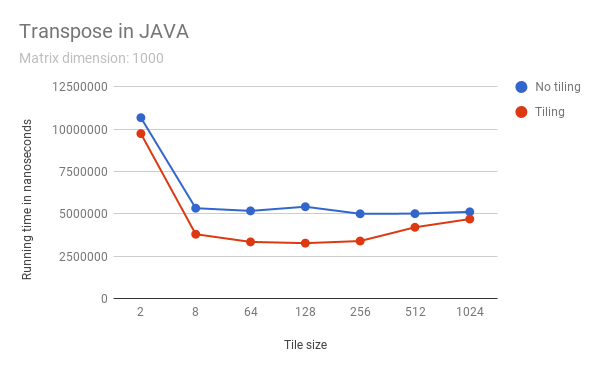
\includegraphics[scale=0.5]{figures/JAVAdifTile1000.png}
\label{fig:JAVA}
\caption{JAVA}
\end{figure}

\begin{figure}
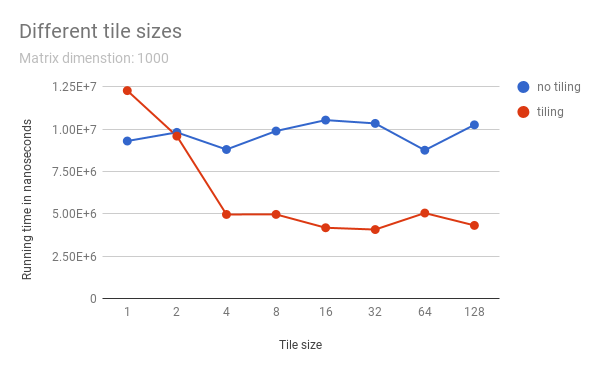
\includegraphics[scale=0.5]{figures/CPPdifTile1000.png}
\label{fig:CPP1k}
\caption{CPP 1k}

\end{figure}

\begin{figure}
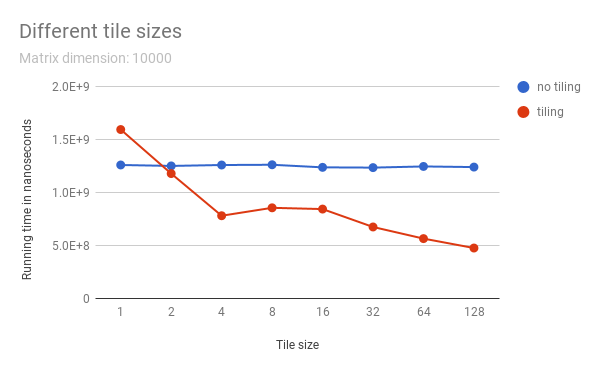
\includegraphics[scale=0.5]{figures/CPPdifTile10000.png}
\label{fig:CPP10k}
\caption{CPP 10k}

\end{figure}

Comparing the performance of the transpose methods on matrices of different sizes in C++ results in the graphs of Figures \ref{fig:CPP} and \ref{fig:CPPlog}.
The running time of the tiling implementation is shorter especially for large input sizes.

\begin{figure}
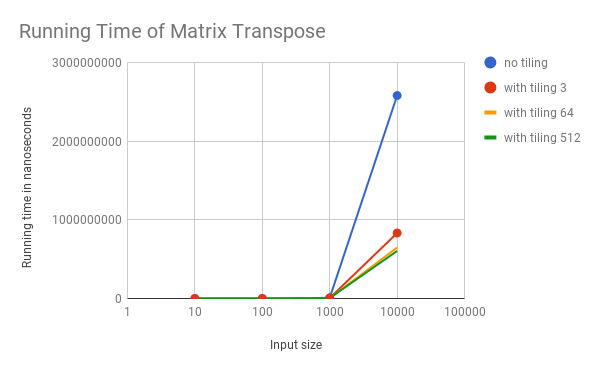
\includegraphics[scale=0.5]{figures/CPPdifInput.png}
\label{fig:CPP}
\caption{CPP}

\end{figure}

\begin{figure}
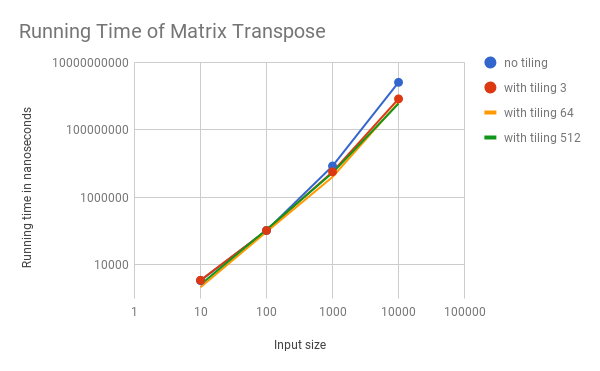
\includegraphics[scale=0.5]{figures/CPPdifInputlog.png}
\label{fig:CPPlog}
\caption{CPP log}

\end{figure}


\section*{Discussion}
In JAVA using tiling did not result in a significant speedup, however the regular implementation of the matrix transpose showed similar runtimes. 
This suggests that the JVM does magic.

In C++ tiling results in better performance even for large tile sizes.

Regarding input size the tiling implementation results in better running time especially for large input sizes.

\end{document}